\chapter{Testing}

\section{Java Unit Tests \& Android Testing Framework}
Die Domain Klassen der RadioTour Applikation enthalten wenig bis gar keine Logik. Aus diesem Grund wird auf herkömmliche \glspl{junit} verzichtet. Als Ersatz werden Tests mit Hilfe des Test Frameworks Robotium 


Da die Programmiersprache für Android Applikationen Java ist, sind \gls{junit} möglich. Android bietet weiter noch ein Testing Framework an, bei welchem gesamte UseCases getestet werden können. In dieser Arbeit gibt es keine vollständige Testabdeckung, da viel Arbeit im User Interface steckt und in der optimalen Anpassung an das Anwendungsumfeld. Dennoch gibt es folgende Testfälle:

\begin{itemize}
\item Testcase 1
\item Testcase 2
\item Testcase 3
\end{itemize}

\section{Feldtest}
Um die Benutzerfreundlichkeit und den Mehrwert der Applikation im Vergleich zur bisherigen Web Applikation zu ermitteln ist ein Feldtest unabdingbar. Es gab die Möglichkeit die \textit{RadioTour} Applikation in einem Berner Fahrrad Rennen zu testen. Bei der Berner Rundfahrt\footnote{Berner Rundfahrt \url{http://www.berner-rundfahrt.ch}} bot sich der  \textit{RadioTour Speaker} der Berner Rundfahrt, David Loosli\footnote{David Loosli, ehemaliger profi Radrennfahrer und \textit{RadioTour Speaker}} der Berner Rundfahrt an, die Applikation zu testen. In einem ersten Treffen wurden die grundlegenden Funktionen der Applikation und die Bedienung erklärt. Weiter ist ein Ausschnitt aus einem fiktiven Rennen durchgespielt worden, wobei eine Person den \gls{chronofunk} simulierte. Ein kurzer Auszug aus der vorbereiteten Situation ist unten aufgeführt.

\begin{itemize}
\item alle Fahrer sind importiert und das Rennen beginnt jetzt
\item Rennzeit wird gestartet
\item \textit{Chronofunk:} Fahrer 4 \& 17 von Beginn an, an der Spitze
\item \textit{Chronofunk:} Bereits 1:07 Vorsprung
\item \textit{Chronofunk:} 31 hat ein defektes Rad und muss raus
\item \textit{Chronofunk:} 8, 83 \& 34 fallen hinter das Feld mit einem Rückstand von 4:31
\end{itemize}

Der vollständige Usability Test sowie der Testlauf an der \textit{Berner Rundfahrt} mit den Rückmeldungen von Herrn Loosli sind im Anhang \ref{ref:usability} zu finden.

Mit den Erfahrungen und den Rückmeldungen aus diesem Event konnte das Endprodukt massiv verbessert werden. Die wesentlichen Punkte die für die Weiterentwicklung verwendet wurden sind:
\begin{itemize}
\item TimePicker Nummern (Auswahl des Rückstandes einer Gruppe) sind zu klein (Korrektur siehe Abbildung \ref{fig:timepicker})
\item nur die Fahrer welche aufgegeben haben oder nicht erschienen sind sollen ausgegraut werden (Vorschlag in Abbildung \ref{fig:riderpicker})
\item ein Fahrer kann folgende Status haben:
\begin{itemize}
\item im Rennen / aktiv
\item nicht gestartet
\item ausgeschieden
\end{itemize}
\item Rennzeit und Kilometer sind nach einem Absturz der Applikation noch verfügbar
\end{itemize}

\begin{figure}[h!]
\caption{TimePicker - Auswahl eines Zeitrückstandes}
\label{fig:timepicker}
\centering
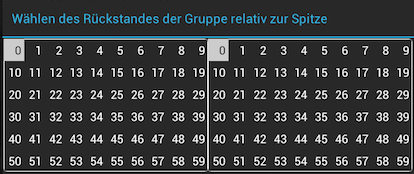
\includegraphics[scale=0.8]{05bericht/images/timepicker.png}
\end{figure} 
Besonders zu hervorheben ist an dieser Stelle, dass Herr Loosli entgegen den Erwartungen die Fahrer, welche in einer Gruppe eingeteilt sind (z.B. Spitze) nicht ausgegraut haben möchte. So entstand der, in Abbildung \ref{fig:riderpicker} dargestellte Entwurf.

\begin{figure}[h!]
\caption{RiderPicker - Auswahl von Fahrern}
\label{fig:riderpicker}
\centering
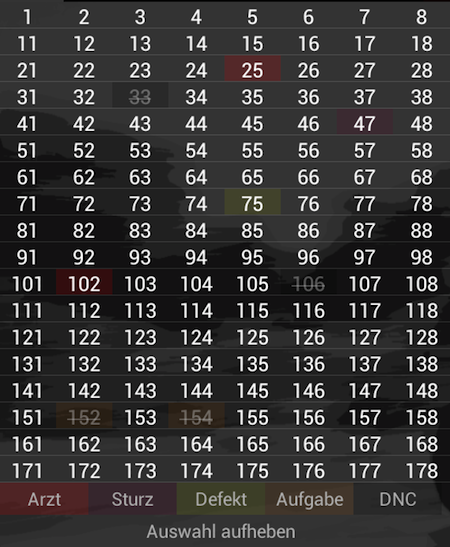
\includegraphics[scale=0.5]{05bericht/images/riderpicker.png}
\end{figure}

Die Abbildung \ref{fig:riderpicker} zeigt eine Situation, bei der die Fahrer 33 und 106 nicht gestartet sind und die Fahrer 152 und 154 aufgegeben haben. Diese Fahrer sind farblich markiert und durchgestrichen. Die weiteren Farben entsprechen den besonderen Ereignissen; Arzt, Sturz oder Defekt eines Fahrers bzw. eines Fahrrads.
